\documentclass[a4paper]{article}

% Version: $Revision: 1.2 $

\usepackage{epsfig}

\newenvironment{tight_itemize}{
\begin{itemize}
  \setlength{\itemsep}{1pt}
  \setlength{\parskip}{0pt}
  \setlength{\parsep}{0pt}}{\end{itemize}
}

\title{
\epsfig{file=images/coat_of_arms.eps,width=10cm}\vspace{3cm}\\WEKA KnowledgeFlow Tutorial\\for Version 3-5-6}
\author{Mark Hall\\Peter Reutemann}

\setcounter{secnumdepth}{3}
\setcounter{tocdepth}{3}

% hyphenation stuff
\hyphenation{Generic-Object-Editor}
\hyphenation{DatabaseUtils}

\begin{document}

\begin{titlepage}

\maketitle
\thispagestyle{empty}

\center
\vspace{8cm}

\copyright 2007 University of Waikato

\end{titlepage}

\tableofcontents

%%%%%%%%%%%%%%%%
% Introduction %
%%%%%%%%%%%%%%%%

\newpage
\section{Introduction}

The KnowledgeFlow provides an alternative to the Explorer as a
graphical front end to WEKA's core algorithms. The KnowledgeFlow is a
work in progress so some of the functionality from the Explorer is not
yet available. On the other hand, there are things that can be done in
the KnowledgeFlow but not in the Explorer.

\begin{center}
	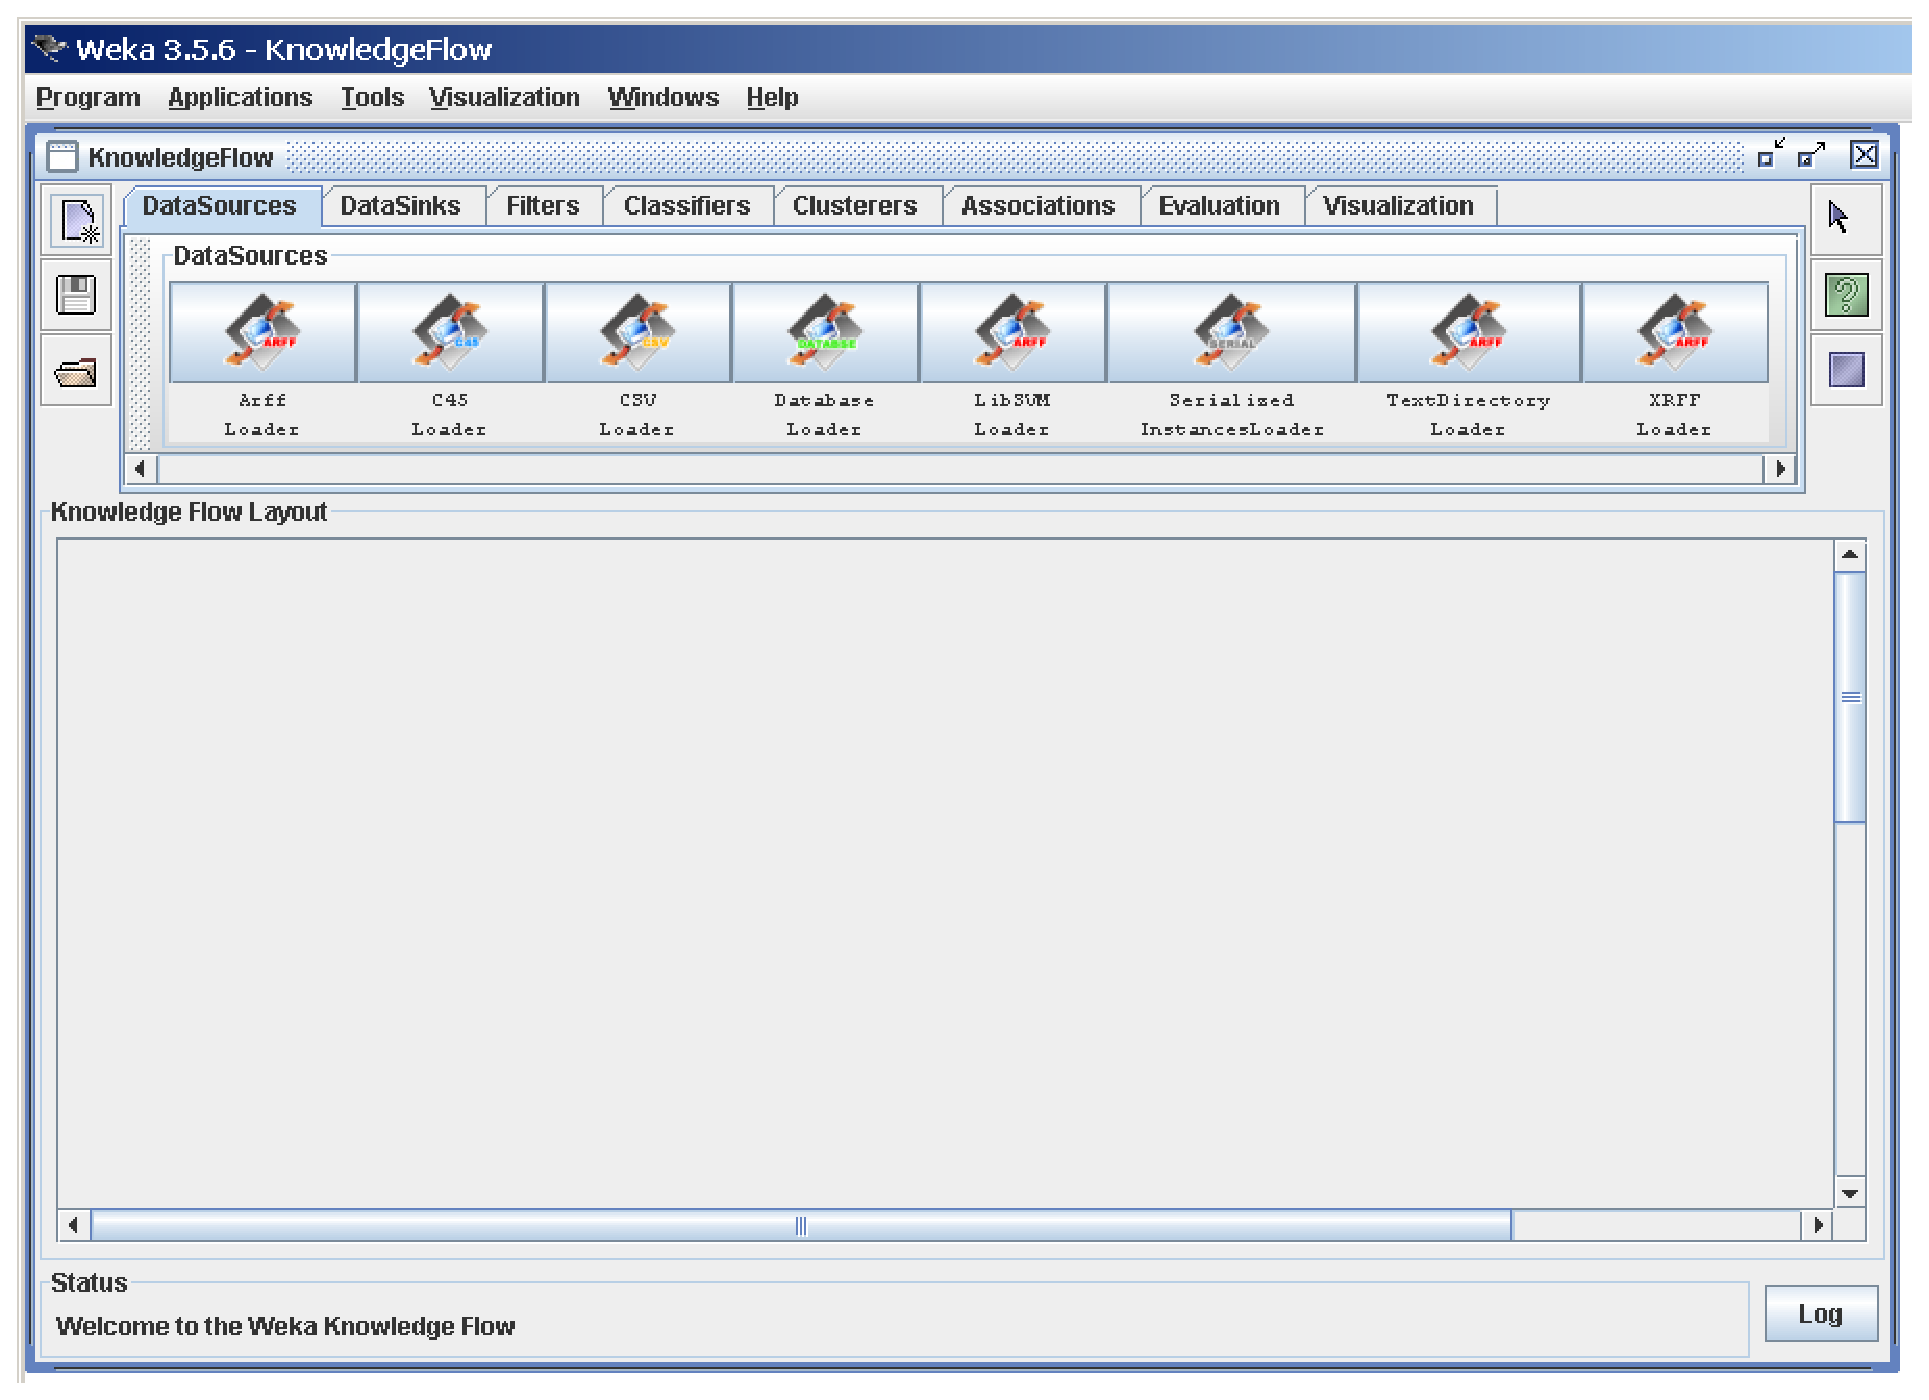
\epsfig{file=images/knowledgeflow.eps,height=7cm}
\end{center}

The KnowledgeFlow presents a \textit{data-flow} inspired interface to
WEKA. The user can select WEKA components from a tool bar, place them
on a layout canvas and connect them together in order to form a
\textit{knowledge flow} for processing and analyzing data. At present, all of
WEKA's classifiers, filters, clusterers, loaders and savers are
available in the KnowledgeFlow along with some extra tools.

The KnowledgeFlow can handle data either incrementally or in batches
(the Explorer handles batch data only). Of course learning from data
incrementally requires a classifier that can be updated on an instance
by instance basis. Currently in WEKA there are ten classifiers that
can handle data incrementally:
\begin{tight_itemize}
	\item AODE
	\item IB1
	\item IBk
	\item KStar
	\item NaiveBayesMultinomialUpdateable
	\item NaiveBayesUpdateable
	\item NNge
	\item Winnow
\end{tight_itemize}

\noindent And two of them are meta classifiers:
\begin{tight_itemize}
	\item \textit{RacedIncrementalLogitBoost} - that can use of any regression base
learner to learn from discrete class data incrementally.
	\item \textit{LWL} - locally weighted learning.
\end{tight_itemize}

\noindent This manual is also available online on the \textit{WekaDoc Wiki} \cite{wekadoc}.

%%%%%%%%%%%%
% Features %
%%%%%%%%%%%%

\newpage
\section{Features}

The KnowledgeFlow offers the following features:
\begin{itemize}
	\item intuitive data flow style layout
	\item process data in batches or incrementally 
	\item process multiple batches or streams in parallel (each separate flow 
  	executes in its own thread)
	\item chain filters together
	\item view models produced by classifiers for each fold in a cross validation
	\item visualize performance of incremental classifiers during 
  	processing (scrolling plots of classification accuracy, RMS error, 
  	predictions etc.)
\end{itemize}

\newpage
\section{Components}
Components available in the KnowledgeFlow:

\subsection{DataSources} All of WEKA's loaders are available.
\begin{center}
	\epsfig{file=images/components_datasources.eps,height=2cm}
\end{center}

\subsection{DataSinks} All of WEKA's savers are available.
\begin{center}
	\epsfig{file=images/components_datasinks.eps,height=2cm}
\end{center}

\subsection{Filters} All of WEKA's filters are available.
\begin{center}
	\epsfig{file=images/components_filters.eps,height=2cm}
\end{center}

\subsection{Classifiers} All of WEKA's classifiers are available.
\begin{center}
	\epsfig{file=images/components_classifiers.eps,height=2cm}
\end{center}

\subsection{Clusterers} All of WEKA's clusterers are available.
\begin{center}
	\epsfig{file=images/components_clusterers.eps,height=2cm}
\end{center}

\subsection{Evaluation}
\begin{center}
	\epsfig{file=images/components_evaluation.eps,height=2cm}
\end{center}

\begin{itemize}
	\item \textit{TrainingSetMaker} - make a data set into a training set.
	\item \textit{TestSetMaker} - make a data set into a test set.
	\item \textit{CrossValidationFoldMaker} - split any data set, training 
	set or test set into folds.
	\item \textit{TrainTestSplitMaker} - split any data set, training set 
	or test set into a training set and a test set.
	\item \textit{ClassAssigner} - assign a column to be the class for any 
	data set, training set or test set.
	\item \textit{ClassValuePicker} - choose a class value to be considered 
	as the ``positive'' class. This is useful when generating data for ROC style 
	curves (see \textit{ModelPerformanceChart} below and example \ref{exampleroc}).
	\item \textit{ClassifierPerformanceEvaluator} - evaluate the performance of 
	batch trained/tested classifiers.
	\item \textit{IncrementalClassifierEvaluator} - evaluate the performance of 
	incrementally trained classifiers.
	\item \textit{ClustererPerformanceEvaluator} - evaluate the performance of 
	batch trained/tested clusterers.
	\item \textit{PredictionAppender} - append classifier predictions to a test 
	set. For discrete class problems, can either append predicted class labels or
	probability distributions.
\end{itemize}

\newpage
\subsection{Visualization}
\begin{center}
	\epsfig{file=images/components_visualization.eps,height=2cm}
\end{center}

\begin{itemize}
	\item \textit{DataVisualizer} - component that can pop up a panel for 
	visualizing data in a single large 2D scatter plot.
	\item \textit{ScatterPlotMatrix} - component that can pop up a panel 
	containing a matrix of small scatter plots (clicking on a small plot 
	pops up a large scatter plot).
	\item \textit{AttributeSummarizer} - component that can pop up a panel 
	containing a matrix of histogram plots - one for each of the attributes 
	in the input data.
	\item \textit{ModelPerformanceChart} - component that can pop up a 
	panel for visualizing threshold (i.e. ROC style) curves.
	\item \textit{TextViewer} - component for showing textual data. Can show 
	data sets, classification performance statistics etc.
	\item \textit{GraphViewer} - component that can pop up a panel for 
	visualizing tree based models.
	\item \textit{StripChart} - component that can pop up a panel that displays 
	a scrolling plot of data (used for viewing the online performance of 
	incremental classifiers).
\end{itemize}

%%%%%%%%%%%%
% Examples %
%%%%%%%%%%%%

\newpage
\section{Examples}

%%%%%%%%%%%%%%%%%%%%%%%%%%%%%%%%
% Example: cross-validated J48 %
%%%%%%%%%%%%%%%%%%%%%%%%%%%%%%%%

\subsection{Cross-validated J48}
Setting up a flow to load an ARFF file (batch mode) and
perform a cross-validation using J48 (WEKA's C4.5 implementation).

\begin{center}
	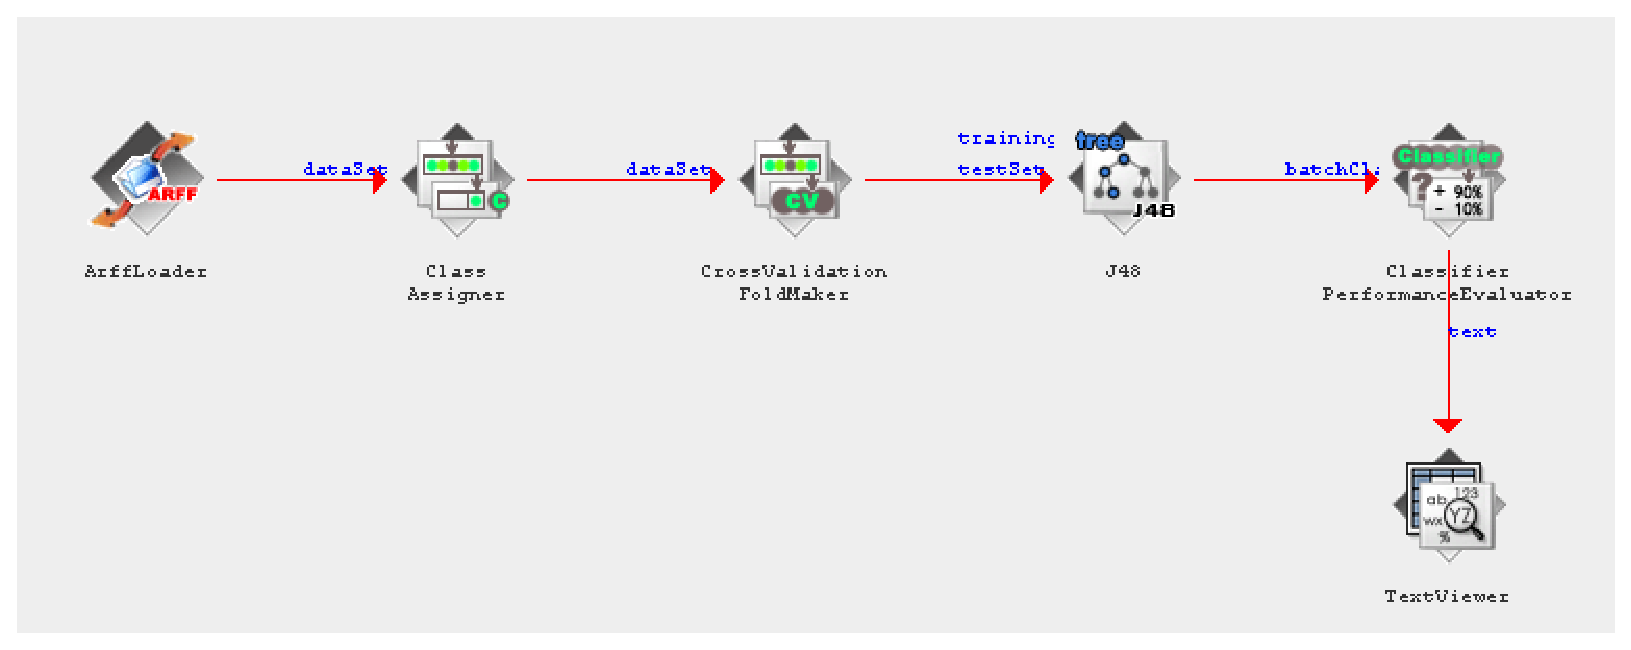
\epsfig{file=images/example_j48.eps,height=4.5cm}
\end{center}

\begin{itemize}
	\item Click on the DataSources tab and choose \textit{ArffLoader} from the
	toolbar (the mouse pointer will change to a \textit{cross hairs}).

	\item Next place the ArffLoader component on the layout area by clicking
	somewhere on the layout (a copy of the ArffLoader icon will appear on
	the layout area).

	\item Next specify an ARFF file to load by first right clicking the mouse
	over the ArffLoader icon on the layout. A pop-up menu will
	appear. Select \textit{Configure} under \textit{Edit} in the list from this menu and
	browse to the location of your ARFF file.

	\item Next click the \textit{Evaluation} tab at the top of the window and choose the
	\textit{ClassAssigner} (allows you to choose which column to be the class)
	component from the toolbar. Place this on the layout.

	\item Now connect the ArffLoader to the ClassAssigner: first right click
	over the ArffLoader and select the \textit{dataSet} under \textit{Connections} in
	the menu. A \textit{rubber band} line will appear. Move the mouse over the
	ClassAssigner component and left click - a red line labeled \textit{dataSet}
	will connect the two components.

	\item Next right click over the ClassAssigner and choose \textit{Configure} from
	the menu. This will pop up a window from which you can specify which
	column is the class in your data (last is the default).

	\item Next grab a \textit{CrossValidationFoldMaker} component from the Evaluation
	toolbar and place it on the layout. Connect the ClassAssigner to the
	CrossValidationFoldMaker by right clicking over \textit{ClassAssigner} and
	selecting \textit{dataSet} from under \textit{Connections} in the menu.

	\item Next click on the \textit{Classifiers} tab at the top of the window and
	scroll along the toolbar until you reach the \textit{J48} component in the
	\textit{trees} section. Place a J48 component on the layout.

	\item Connect the CrossValidationFoldMaker to J48 TWICE by first choosing
	\textit{trainingSet} and then \textit{testSet} from the pop-up menu for the
	CrossValidationFoldMaker.

	\item Next go back to the \textit{Evaluation} tab and place a
	\textit{ClassifierPerformanceEvaluator} component on the layout. Connect J48
	to this component by selecting the \textit{batchClassifier} entry from the
	pop-up menu for J48.

	\item Next go to the \textit{Visualization} toolbar and place a \textit{TextViewer}
	component on the layout. Connect the ClassifierPerformanceEvaluator to
	the TextViewer by selecting the \textit{text} entry from the pop-up menu for
	ClassifierPerformanceEvaluator.

	\item Now start the flow executing by selecting \textit{Start loading} from the
	pop-up menu for ArffLoader. Depending on how big the data set is and
	how long cross-validation takes you will see some animation from some
	of the icons in the layout (J48's tree will \textit{grow} in the icon and the
	ticks will animate on the ClassifierPerformanceEvaluator). You will
	also see some progress information in the \textit{Status} bar and \textit{Log} at
	the bottom of the window.
\end{itemize}

When finished you can view the results by choosing \textit{Show results} from
the pop-up menu for the \textit{TextViewer} component.

Other cool things to add to this flow: connect a \textit{TextViewer} and/or a
\textit{GraphViewer} to J48 in order to view the textual or graphical
representations of the trees produced for each fold of the cross
validation (this is something that is not possible in the Explorer).

%%%%%%%%%%%%%%%%%%%%%%%%%
% Example: multiple ROC %
%%%%%%%%%%%%%%%%%%%%%%%%%

\newpage
\subsection{Plotting multiple ROC curves}
\label{exampleroc}
The KnowledgeFlow can draw multiple ROC curves in the same plot window, something that the 
Explorer cannot do. In this example we use \textit{J48} and \textit{RandomForest}
as classifiers. This example can be found on the \textit{WekaWiki} as well \cite{multipleroc}.

\begin{center}
	\epsfig{file=images/example_multiple_roc.eps,height=4cm}
\end{center}

\begin{itemize}
	\item Click on the DataSources tab and choose \textit{ArffLoader} from the
	toolbar (the mouse pointer will change to a \textit{cross hairs}).

	\item Next place the ArffLoader component on the layout area by clicking
	somewhere on the layout (a copy of the ArffLoader icon will appear on
	the layout area).

	\item Next specify an ARFF file to load by first right clicking the mouse
	over the ArffLoader icon on the layout. A pop-up menu will
	appear. Select \textit{Configure} under \textit{Edit} in the list from this menu and
	browse to the location of your ARFF file.

	\item Next click the \textit{Evaluation} tab at the top of the window and choose the
	\textit{ClassAssigner} (allows you to choose which column to be the class)
	component from the toolbar. Place this on the layout.

	\item Now connect the ArffLoader to the ClassAssigner: first right click
	over the ArffLoader and select the \textit{dataSet} under \textit{Connections} in
	the menu. A \textit{rubber band} line will appear. Move the mouse over the
	ClassAssigner component and left click - a red line labeled \textit{dataSet}
	will connect the two components.

	\item Next right click over the ClassAssigner and choose \textit{Configure} from
	the menu. This will pop up a window from which you can specify which
	column is the class in your data (last is the default).

	\item Next choose the \textit{ClassValuePicker} (allows you to choose which class 
	label to be evaluated in the ROC) component from the toolbar. Place this on the layout
	and right click over \textit{ClassAssigner} and select \textit{dataSet} from under
	\textit{Connections} in the menu and connect it with the \textit{ClassValuePicker}.

	\item Next grab a \textit{CrossValidationFoldMaker} component from the Evaluation
	toolbar and place it on the layout. Connect the ClassAssigner to the
	CrossValidationFoldMaker by right clicking over \textit{ClassAssigner} and
	selecting \textit{dataSet} from under \textit{Connections} in the menu.

	\item Next click on the \textit{Classifiers} tab at the top of the window and
	scroll along the toolbar until you reach the \textit{J48} component in the
	\textit{trees} section. Place a J48 component on the layout.

	\item Connect the CrossValidationFoldMaker to J48 TWICE by first choosing
	\textit{trainingSet} and then \textit{testSet} from the pop-up menu for the
	CrossValidationFoldMaker.

	\item Repeat these two steps with the RandomForest classifier.

	\item Next go back to the \textit{Evaluation} tab and place a
	\textit{ClassifierPerformanceEvaluator} component on the layout. Connect J48
	to this component by selecting the \textit{batchClassifier} entry from the
	pop-up menu for J48. Add another \textit{ClassifierPerformanceEvaluator} for
	RandomForest and connect them via \textit{batchClassifier} as well.

	\item Next go to the \textit{Visualization} toolbar and place a 
	\textit{ModelPerformanceChart} component on the layout. Connect both 
	ClassifierPerformanceEvaluators to the ModelPerformanceChart by selecting 
	the \textit{thresholdData} entry from the pop-up menu for ClassifierPerformanceEvaluator.

	\item Now start the flow executing by selecting \textit{Start loading} from the
	pop-up menu for ArffLoader. Depending on how big the data set is and
	how long cross validation takes you will see some animation from some
	of the icons in the layout. You will also see some progress information in the 
	\textit{Status} bar and \textit{Log} at the bottom of the window.
	
	\item Select \textit{Show plot} from the popup-menu of the 
	\textit{ModelPerformanceChart} under the \textit{Actions} section.
\end{itemize}

Here are the two ROC curves generated from the UCI dataset \textit{credit-g}, 
evaluated on the class label \textit{good}:

\begin{center}
	\epsfig{file=images/example_multiple_roc_output.eps,height=8.5cm}
\end{center}

\newpage
\begin{thebibliography}{999}
	\bibitem{witten} Witten, I.H. and Frank, E. (2005) \textit{Data Mining: Practical machine
learning tools and techniques. 2nd edition}  Morgan Kaufmann, San
Francisco.
	\bibitem{wekadoc} \textit{WekaDoc} -- \texttt{http://weka.sourceforge.net/wekadoc/}
	\bibitem{wekawiki} \textit{WekaWiki} -- \texttt{http://weka.sourceforge.net/wekawiki/}
	\bibitem{multipleroc} \textit{Plotting multiple ROC curves} on \textit{WekaWiki} -- \\
\small{\texttt{http://weka.sourceforge.net/wiki/index.php/Plotting\_multiple\_ROC\_curves}}
\end{thebibliography}

\end{document}
